\documentclass{bmstu}

\bibliography{biblio}

\begin{document}

\makecourseworktitle
    {Информатика, искусственный интеллект и системы управления} % Название факультета
    {Программное обеспечение ЭВМ и информационные технологии} % Название кафедры
    {Драйвер устройства сканирования отпечатков пальцев Shenzhen Goodix Technology для операционной системы Linux} % Тема работы
    {Корниенко~К.~Ю./ИУ7-71Б} % Номер группы/ФИО студента (если авторов несколько, их необходимо разделить запятой)
    {Рязанова~Н.~Ю.} % ФИО научного руководителя
    {} % ФИО консультанта (необязательный аргумент; если консультантов несколько, их необходимо разделить запятой)

\maketableofcontents

\chapter*{ВВЕДЕНИЕ}
\addcontentsline{toc}{chapter}{ВВЕДЕНИЕ}

Цель данной работы --- написать драйвер сканера отпечатка пальца.

\chapter{Аналитический раздел}

\section{Постановка задачи}

В соответствии с техническим заданием, требуется написать драйвер сканера отпечатка пальца Shenzhen Goodix Technology \cite{goodix} для операционной системы Linux.

Для решения поставленной задачи необходимо:

\begin{itemize}[label=---]
    \item проанализировать особенности работы сканера отпечатка пальца;
    \item рассмотреть способы получения данных от устройства с использованием подсистемы USB \cite{USB};
    \item разработать драйвер в виде загружаемого модуля ядра;
    \item провести исследование разработанного драйвера.
\end{itemize}

\section{Конфигурация устройства}

Ниже приведена конфигурация устройства, полученная из отладочной файловой системы по пути \texttt{/sys/kernel/debug/devices} \cite{sysfs}.

\begin{verbatim}
T:  Bus=03 Lev=01 Prnt=01 Port=03 Cnt=01 Dev#=  2 Spd=12   MxCh= 0
D:  Ver= 2.00 Cls=02(comm.) Sub=01 Prot=01 MxPS=64 #Cfgs=  1
P:  Vendor=27c6 ProdID=5125 Rev= 2.00
S:  Manufacturer=Shenzhen Goodix Technology Co.,Ltd.
S:  Product=Goodix Fingerprint Device
S:  SerialNumber=00000000001A
C:* #Ifs= 2 Cfg#= 1 Atr=60 MxPwr=100mA
I:* If#= 0 Alt= 0 #EPs= 1 Cls=02(comm.) Sub=01 Prot=01 Driver=(none)
E:  Ad=82(I) Atr=03(Int.) MxPS=   8 Ivl=16ms
I:* If#= 1 Alt= 0 #EPs= 2 Cls=0a(data ) Sub=00 Prot=00 Driver=(none)
E:  Ad=01(O) Atr=02(Bulk) MxPS=  64 Ivl=0ms
E:  Ad=81(I) Atr=02(Bulk) MxPS=  64 Ivl=0ms
\end{verbatim}

Данное устройство имеет одну конфигурацию с двумя активными интерфейсами, первый из которых предназначен для передачи управляющих комманд, а второй -- для передачи данных.

\section{Подсистема USB}

USB драйвер имеет две точки входа -- \texttt{probe} и \texttt{disconnect} \cite{usb-driver}, которые вызываются подсистемой USB при подключении и отключении устройства, соответствующего данному драйверу.

Обмен информацией между подключенным устройством и драйвером осуществляется пакетами по запросу. Блок запроса USB (USB Request Block -- URB) представляется структурой ядра \texttt{urb}:

\begin{small}
\begin{verbatim}
struct urb {
    struct list_head urb_list;
    struct usb_device *dev; /* (in) pointer to associated device */
    unsigned int pipe; /* (in) pipe information */
    int status; /* (return) non-ISO status */
    void *transfer_buffer; /* (in) associated data buffer */
    dma_addr_t transfer_dma; /* (in) dma addr for transfer_buffer */
    u32 transfer_buffer_length; /* (in) data buffer length */
    u32 actual_length; /* (return) actual transfer length */
    int interval; /* (modify) transfer interval */
    void *context; /* (in) context for completion */
    usb_complete_t complete; /* (in) completion routine */
    /* ... */
};
\end{verbatim}
\end{small}

\subsection{Способы передачи URB пакетов}

Передача URB пакетов по шине USB является дуплексной и может происходить в одной из четырех форм, в зависимости от подключенного устройства:

\begin{itemize}[leftmargin=1.6\parindent]
    \item[---] \texttt{Control} -- используется для передачи управляющих команд для настройки устройства или получения его статуса.
    \item[---] \texttt{Bulk} -- используется для обмена большими пакетами данных. Зачастую именно эта форма передачи используется устройствами на подобие сканеров и SCSI адаптеров.
    \item[---] \texttt{Interrupt} -- используется для запроса передачи небольших пакетов в режиме опроса устройства. Если был запрошен пакет в режиме прерывания, то драйвер хост-контроллера автоматически будет повторять этот запрос с определенным интервалом (1--255 мс).
    \item[---] \texttt{Isochronous} -- используется для передачи данных в реальном времени с гарантированной пропускной способностью шины, но ненадежно. В общем случае изохронный тип используется для передачи аудио и видео информации. 
\end{itemize}

Рассматриваемое устройство -- сканер отпечатка пальца -- поддерживает форматы передачи \texttt{Control} (для передачи управляющих команд) и \texttt{Bulk} (для передачи изображения считанного отпечатка пальца).

\section{Особенности взаимодействия с устройством с использованием протокола TLS}

Сканер отпечатков пальцев Shenzhen Goodix Technology для Linux требует использования протокола TLS \cite{tls} 1.2 для защиты передачи данных.

Для аутентификации в данном протоколе используются асимметричные алгоритмы
шифрования \cite{encryption} (открытый ключ -- закрытый ключ), а для сохранения конфиденциальности --
симметричные (с одним, секретным, ключом), также используются и сеансовые ключи, которые
необходимы для каждого отдельного уникального защищенного сеанса.

В соответствии с протоколом TLS процесс инициации сеанса, также называемый <<рукопожатием>>, состоит из следующих шагов:

\begin{enumerate}
    \item Клиент (в данном случае -- драйвер) отправляет запрос на безопасное соединение с сервером (устройством).
    \item Сервер предоставляет цифровой сертификат, подтверждающий подлинность сервера.
    \item Используя открытый ключ сервера, клиент и сервер устанавливают сеансовый ключ, с помощью которого шифруются данные на протяжении всего сеанса.
\end{enumerate}

Установка защищенного соединение с устройством производится через отправку URB Control блоков.

\section{Взаимодействие драйвера с пользовательскими программами}

Одним из возможных способов передачи информации из пространства ядра в пространство пользователя является использование виртуальной файловой системы proc \cite{vfs-proc}.

Операции, которые могут быть осуществлены с файлом определяются структурой \texttt{proc\_ops}. В данной работе необходимо и достаточно реализовать следующие операции: \texttt{proc\_open}, \texttt{proc\_read}, \texttt{proc\_lseek}, \texttt{proc\_poll}, \texttt{proc\_release}.

Так как изображение отпечатка пальца имеет существенный размер, пользовательское приложение может не обработать все данные за одну операцию чтения.
В ядре Linux есть интерфейс файлов последовательностей (sequence file).
Использование данного интерфейса избавляет разработчика загружаемого модуля ядра от необходимости учитывать описанную проблему.


В случае, если пользователь не прикладывает палец к сканеру, процесс должен быть заблокирован при попытке чтения. Необходимость блокировки процесса и ожидания появления нового события приводит к использованию очередей ожидания, которые представляются в ядре структурой \texttt{wait\_queue\_head}:

\begin{small}
\begin{verbatim}
struct wait_queue_entry {
    unsigned int flags;
    void *private;
    wait_queue_func_t func;
    struct list_head entry;
};

struct wait_queue_head {
    spinlock_t lock;
    struct list_head head;
};
\end{verbatim}
\end{small}

Блокировка процесса и ожидание возникновения события осуществляется вызовом макроса

\texttt{wait\_event\_interruptible(wq\_head, condition)}.

Все ждущие в данной очереди процессы пробуждаются посредством вызова макроса \texttt{wake\_up\_all(wq\_head)}, после чего будет анализировано выражение \texttt{condition} переданное при блокировке. Если оно ложно, то процесс вновь блокируется.

Для поддержки механизма опроса реализуется функция \texttt{proc\_poll}.

\subsection*{Выводы}

В данном разделе была представлена конфигурация устройства сканера, изложены основные моменты работы с подсистемой USB при проектировании драйверов USB-устройств в ОС Linux. Также рассмотрены особенности взаимодействия драйвера с устройством с использованием протокола TLS и обеспечением защищенного соединения. Обсуждены способы передачи данных из пространства ядра в пространство пользователя.


\chapter{Конструкторский раздел}

В данном разделе приведены ключевые алгоритмы использованные при написании драйвера сканера отпечатка пальца.

\section{Структура ПО}

Разрабатываемое ПО состоит из драйвера сканера отпечатка пальца и пользовательского приложения для тестирования работы драйвера.

\begin{figure}[h!]
    \centering
    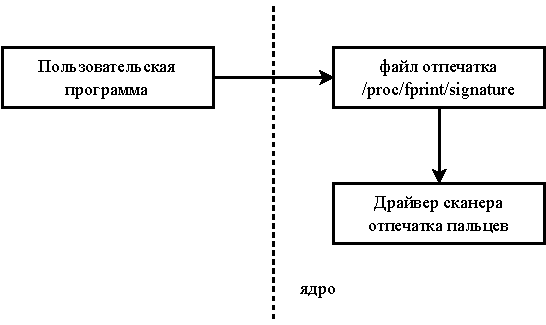
\includegraphics[width=0.9\textwidth]{img/structure-po}
    \caption{Структура ПО}
\end{figure}

\clearpage

\section{Алгоритм инициализации TLS-соединения}

На рисунке \ref{fig:init} представлен алгоритм инициализации TLS соединения с устройством. PSK \cite{psk} -- pre-shared key ciphersuites -- предварительный общий ключ безопасности используемый в качестве сертификата.

\begin{figure}[h!]
    \centering
    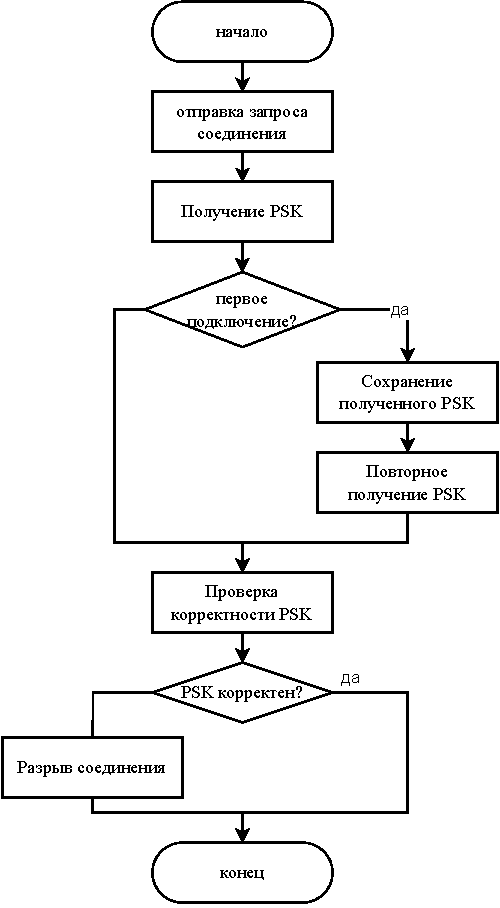
\includegraphics[width=0.6\textwidth]{img/init}
    \caption{Алгоритм инициализации соединения}
    \label{fig:init}
\end{figure}

\clearpage

\section{Обработка пользовательских запросов}

Сканер отпечатков пальцев является общим ресурсом для всех пользовательских приложений. Разрабатывая драйвер данного устройства важно рассмотреть все проблемы, которые могут возникнуть при обращении к драйверу различными пользовательскими приложениями в многопоточной системе.
Множество возможных проблем включает в себя следующие: 

\begin{enumerate}
    \item несколько пользовательских программ могут одновременно запрашивать отпечаток;
    \item несколько потоков одного процесса могут запрашивать отпечаток;
    \item процесс(поток) может умереть недочитав отпечаток;
    \item процесс(поток) может недочитать отпечаток.
\end{enumerate}

В качестве решения для указанных проблем можно предложить следующие подходы.

Во-первых, для обеспечения эффективной синхронизации захвата и использования ресурсов сканера отпечатков пальцев могут быть применены мьютексы, которые позволят ограничить доступ к общему ресурсу только одному потоку или процессу в определенный момент времени.

Кроме того, для решения проблемы прерванного чтения отпечатков пальцев можно ввести механизм отслеживания времени, чтобы по истечении определенного периода запрос отпечатка пальца был принудительно завершен. Это позволит избежать затянутого доступа к ресурсу в случае, если пользовательское приложение не успевает оперативно обработать данные от сканера.

Таким образом, разработка драйвера для сканера отпечатков пальцев в многопоточной системе требует учета и обработки указанных проблем с использованием вышеуказанных решений.

\clearpage

\section{Взаимодействие с ФС proc}

В контексте разработки драйвера сканера отпечатка пальцев важно иметь возможность передавать считанный отпечаток из пространства ядра в пространство пользователя. Для этого можно использовать интерфейс файлов последовательностей, предоставляемый ядром Linux. При этом данные считанного отпечатка будут представлены как последовательность байт, которую можно передать из пространства ядра в пространство пользователя с помощью файлов в виртуальной файловой системе \texttt{proc}. Диаграмма вызовов функций, определенных на \texttt{seq\_file} представлена на рисунке \ref{fig:seq-file}.

\begin{figure}[h!]
    \centering
    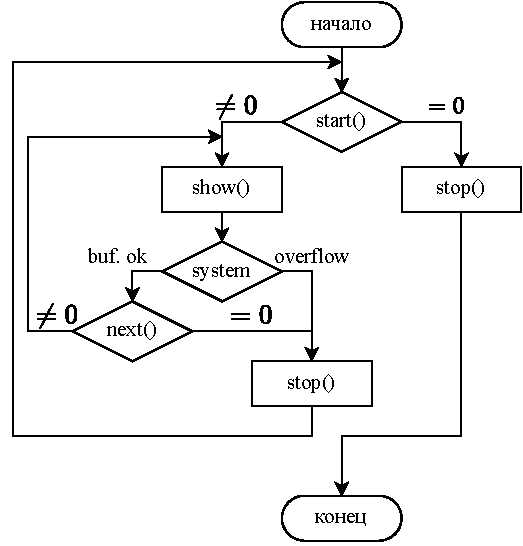
\includegraphics[width=0.7\linewidth]{img/seq-file.pdf}
    \caption{Диаграмма вызовов функций, определенных на \texttt{seq\_file}}
    \label{fig:seq-file}
\end{figure}

Альтернативными способами передачи отпечатка из пространства ядра в пространство пользователя могут быть использование специальных функций ядра, таких как \texttt{copy\_to\_user()} или системного вызова \texttt{mmap()}.

\clearpage

В случае разработки драйвера сканера отпечатка пальцев, использование интерфейса файлов последовательностей обосновано тем, что они предоставляют удобный механизм для передачи последовательности данных из ядра в пространство пользователя. Кроме того, они позволяют удобно осуществлять чтение и запись данных с использованием стандартных интерфейсов файловой системы, что упрощает взаимодействие пользовательских программ с драйвером сканера отпечатка пальцев.

\clearpage

\chapter{Технологический раздел}

\section{Выбор языка и среды разработки}

Для написания драйвера был выбран язык программирования C.

Для сборки драйвера будет использована утилита Make. В качестве среды разработки был выбран редактор VSCode.

Драйвер разрабатывается для ОС Linux версии 6.7.

\section{Точки входа драйвера}

\begin{lstlisting}[caption={функция \texttt{probe} драйвера}]
int fprint_probe(struct usb_interface *intf, const struct usb_device_id *id)
{
    printk(KERN_INFO LOG_PREFIX "fingerprint usb interface probed\n");

    struct usb_host_interface *iface = intf->cur_altsetting;
    printk(KERN_INFO LOG_PREFIX "fingerprint usb interface number: %d\n", iface->desc.bInterfaceNumber);
    if (iface->string != NULL) {
        printk(KERN_INFO LOG_PREFIX "fingerprint usb interface string: %s\n", iface->string);
    } else {
        printk(KERN_WARNING LOG_PREFIX "fingerprint usb interface string is NULL\n");
    }

    if (iface->desc.bNumEndpoints != 3) {
        printk(KERN_INFO LOG_PREFIX "skipping this interface\n");
        return 0;
    }

    if (iface->desc.bInterfaceNumber != 0) {
        printk(KERN_INFO LOG_PREFIX "skipping this interface\n");
        return 0;
    }

    struct usb_endpoint_descriptor *endpoint = &iface->endpoint[0].desc;
    if (endpoint->bEndpointAddress != 0x82) {
        printk(KERN_WARNING LOG_PREFIX "endpoint[1] must have adress 0x81\n");
        return 0;
    }

    int res = initialize_fprint_endpoint(intf, endpoint);
    if (res != 0) {
        printk(KERN_ERR LOG_PREFIX "failed to initialize endpoint\n");
    }
    return res;
}
\end{lstlisting}

\begin{lstlisting}[caption={функция \texttt{disconnect} драйвера}]
void fprint_disconnect(struct usb_interface *intf)
{
    printk(KERN_INFO LOG_PREFIX "fingerprint usb interface disconnected\n");

    struct usb_host_interface *iface = intf->cur_altsetting;
    printk(KERN_INFO LOG_PREFIX "fingerprint usb interface number: %d\n", iface->desc.bInterfaceNumber);
    printk(KERN_INFO LOG_PREFIX "fingerprint usb interface string: %d\n", iface->desc.iInterface);

    // free allocated structures here
    if (iface->desc.bInterfaceNumber != 0) {
        printk(KERN_INFO LOG_PREFIX "skipping this interface\n");
        return;
    }

    struct usb_endpoint_descriptor *endpoint = &iface->endpoint[0].desc;
    if (endpoint->bEndpointAddress != 0x82) {
        printk(KERN_WARNING LOG_PREFIX "endpoint[1] must have adress 0x81\n");
        return;
    }

    struct usb_device* usbdev = interface_to_usbdev(intf);
    struct fprint_drv_data* drvdata = dev_get_drvdata(&usbdev->dev);
    if (drvdata != NULL) {
        // usb_free_urb(drvdata->urb);
        kfree(drvdata->transfer_buffer);
        kfree(drvdata);
        printk(KERN_INFO LOG_PREFIX "driver data free'd\n");
    }
}
\end{lstlisting}

\section{Работа с файловой системой proc}

\begin{lstlisting}[caption={функции работы с VFS proc}]
static atomic_t reader_available = ATOMIC_INIT(1);
static DECLARE_WAIT_QUEUE_HEAD(reader_queue);
static DECLARE_WAIT_QUEUE_HEAD(poll_wait_queue);

static const struct seq_operations fprint_seq_ops = {
    .start = start,
    .next = next,
    .stop = stop,
    .show = show
};

static const struct proc_ops fprint_proc_ops = {
    .proc_open    = open,
    .proc_read    = seq_read,
    .proc_lseek   = seq_lseek,
    .proc_release = seq_release,
    .proc_poll    = poll,
};

void* start(struct seq_file *m, loff_t *pos)
{
    seqfile_iterator = 0;
    return &seqfile_iterator;
}

void stop(struct seq_file *m, void *v)
{
    atomic_set(&reader_available, 1);
}

void* next(struct seq_file *m, void *v, loff_t *pos)
{
    wait_event_interruptible(reader_queue, signature_data_available);
    signature_data_available = false;

    *pos += signature_data_size;
    return NULL;
}

int show(struct seq_file *m, void *v)
{
    if (signature_data == NULL) {
        printk(KERN_WARNING LOG_PREFIX "signature data is NULL\n");
        return 0;
    }

    seq_write(m, signature_data, signature_data_size);
    return 0;
}

int open(struct inode* inode, struct file* file)
{
    signature_data_available = false;
    return seq_open(file, &fprint_seq_ops);
}

static unsigned int poll(struct file *file, poll_table *wait)
{
    poll_wait(file, &poll_wait_queue, wait);
    if (signature_data_available)
        return POLLIN | POLLRDNORM;
    return 0;
}
\end{lstlisting}

\chapter{Исследовательский раздел}

\section{Постановка исследования}

Исследование скорости обработки запроса отпечатка пальца было проведено для значений размера буфера чтения от 16 до 512 байт. Замер времени осуществлялся с использованием функции \texttt{clock\_gettime} стандартной библиотеки языка С. При этом в качестве идентификатора часов использовался \texttt{CLOCK\_PROCESS\_CPUTIME\_ID} для измерения времени, затраченного непосредственно процессом.

\section{Результаты}

На рисунке \ref{fig:research} приведен график зависимости времени обработки запроса отпечатка пальца пользовательского приложения от размера буфера чтения.

\begin{figure}[h!]
    \centering
    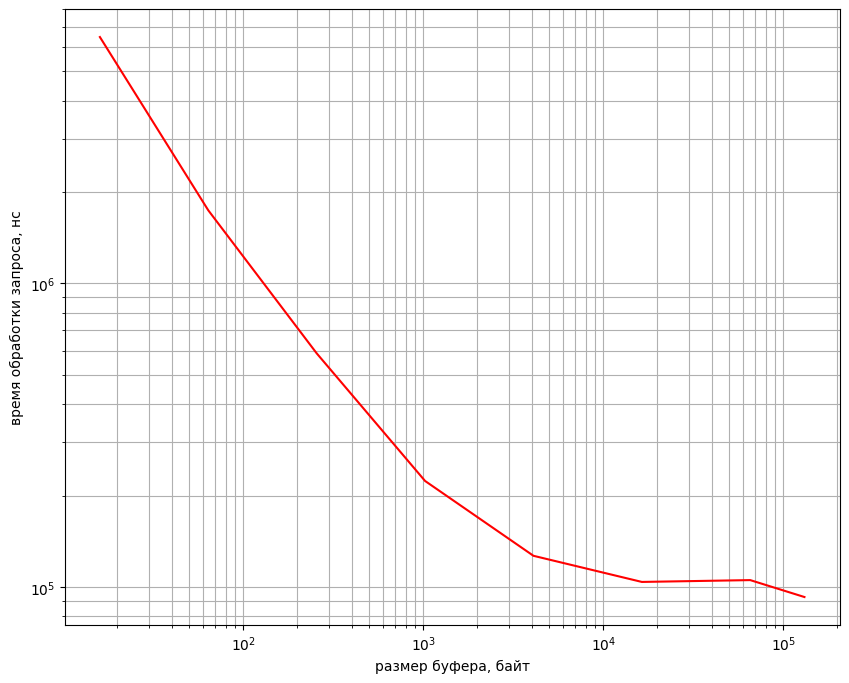
\includegraphics[width=\textwidth]{img/research.png}
    \caption{Зависимость времени обработки запроса от размера буфера}
    \label{fig:research}
\end{figure}

\chapter*{ЗАКЛЮЧЕНИЕ}
\addcontentsline{toc}{chapter}{ЗАКЛЮЧЕНИЕ}

В ходе работы была изучена подсистема USB, рассмотрены и решены проблемы связанные с работой сканера отпечатка пальца.

Был разработан драйвер для сканера отпечатка пальцев.

Было проведено исследование зависимости времени обработки запроса отпечатка пальца от пользовательского приложения для различных размеров буферов.


\makebibliography

\begin{appendices}
	\chapter{}
\end{appendices}

\end{document}